
\begin{figure}[t]
	\centering
	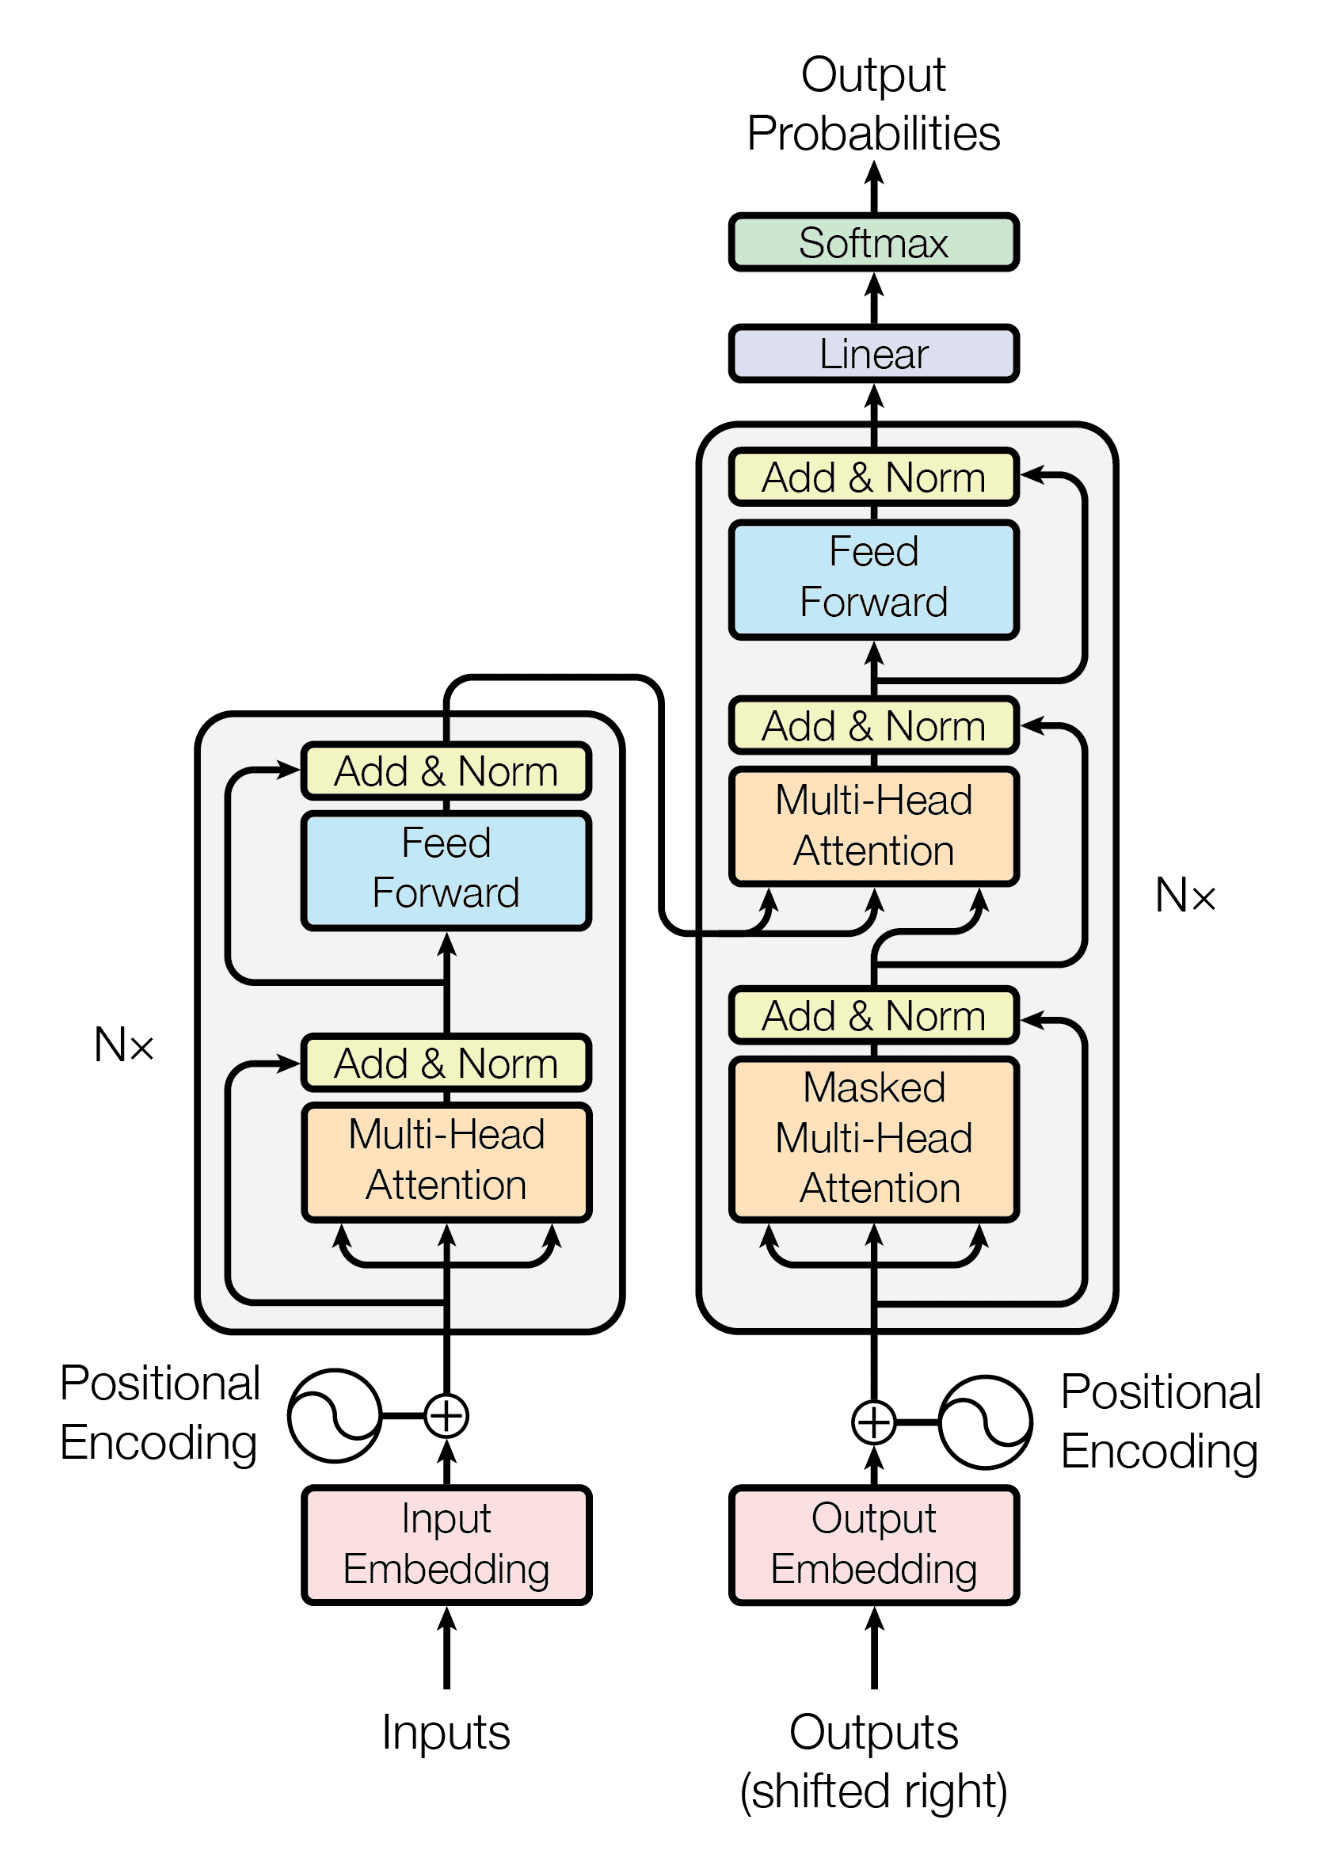
\includegraphics[scale=0.2]{./images/transformer/transformer.png}
	\caption{An illustration of Transformer architecture.}
\end{figure}

\paragraph{TLDR}
\begin{itemize}
	\item \textit{Attention is a communication mechanism}, which can be seen as nodes in a directed graph looking at each other and aggregating information with a weighted sum from all nodes that point to them, with data-dependent weights.
	\item There is no notion of space. Attention simply acts over a set of vectors. This is why we need to positionally encode tokens.
	\item Each example across batch dimension is of course processed completely independently and never ``talk'' to each other
	\item In an ``encoder'' attention block just delete the single line that does masking with `tril`, allowing all tokens to communicate. This block here is called a ``decoder'' attention block because it has triangular masking, and is usually used in autoregressive settings, like language modeling.
	\item ``self-attention'' just means that the keys and values are produced from the same source as queries. In ``cross-attention'', the queries still get produced from $x$, but the keys and values come from some other, external source (\eg an encoder module)
	\item ``Scaled'' attention additional divides `wei` by $1/sqrt(head\_size)$. This makes it so when input Q,K are unit variance, wei will be unit variance too and Softmax will stay diffuse and not saturate too much. Illustration below
\end{itemize}

\section{Attention Mechanism}
\label{sec:nlp_attention}


The attention mechanism assigns \textit{attention scores} (\ie \textit{weights}) to different parts of the input sequence, indicating how much each part contributes to the current output. In essence, the model ``pays attention'' to certain parts of the input more than others while processing each token in the sequence.

Assume the encoder produces 3 hidden states (each a 2-dimensional vector):
\[
h_1 = \begin{bmatrix} 1 \\ 0 \end{bmatrix}, \quad
h_2 = \begin{bmatrix} 0 \\ 1 \end{bmatrix}, \quad
h_3 = \begin{bmatrix} 1 \\ 1 \end{bmatrix}.
\]

Let the decoder’s previous hidden state at time \( t-1 \) be:
\[
s_{t-1} = \begin{bmatrix} 0.5 \\ 0.2 \end{bmatrix}.
\]

Using the \textit{dot product} as our score function, the alignment score for each encoder hidden state is:
\[
e_{tj} = s_{t-1}^\top h_j.
\]

Compute each:
\begin{enumerate}
	\item  For \( h_1 \):
   \[
   e_{t1} = [0.5 \quad 0.2] \cdot \begin{bmatrix} 1 \\ 0 \end{bmatrix} = 0.5.
   \]
\item For \( h_2 \):
   \[
   e_{t2} = [0.5 \quad 0.2] \cdot \begin{bmatrix} 0 \\ 1 \end{bmatrix} = 0.2.
   \]
\item For \( h_3 \):
   \[
   e_{t3} = [0.5 \quad 0.2] \cdot \begin{bmatrix} 1 \\ 1 \end{bmatrix} = 0.7.
   \]
\end{enumerate}

The attention weight for each encoder time step is given by:
\[
\alpha_{tj} = \frac{\exp(e_{tj})}{\sum_{k=1}^{3} \exp(e_{tk})}.
\]

Calculate the exponentials:
\begin{itemize}
	\item \(\exp(0.5) \approx 1.6487\),
	\item \(\exp(0.2) \approx 1.2214\),
	\item \(\exp(0.7) \approx 2.0138\).
\end{itemize}

Sum of exponentials:
\[
S = 1.6487 + 1.2214 + 2.0138 \approx 4.8839.
\]

Now compute each attention weight:
\begin{enumerate}
	\item For \( \alpha_{t1} \):
   \[
   \alpha_{t1} = \frac{1.6487}{4.8839} \approx 0.3374.
   \]
\item For \( \alpha_{t2} \):
   \[
   \alpha_{t2} = \frac{1.2214}{4.8839} \approx 0.2501.
   \]
\item For \( \alpha_{t3} \):
   \[
   \alpha_{t3} = \frac{2.0138}{4.8839} \approx 0.4125.
   \]
\end{enumerate}

These weights sum to 1 (up to rounding):

\[
0.3374 + 0.2501 + 0.4125 \approx 1.0000.
\]

The context vector \( c_t \) is the weighted sum of the encoder hidden states:

\[
c_t = \alpha_{t1} h_1 + \alpha_{t2} h_2 + \alpha_{t3} h_3.
\]

Substitute in the values:

\[
\begin{aligned}
c_t &= 0.3374 \begin{bmatrix} 1 \\ 0 \end{bmatrix} 
+ 0.2501 \begin{bmatrix} 0 \\ 1 \end{bmatrix} 
+ 0.4125 \begin{bmatrix} 1 \\ 1 \end{bmatrix} \\
&= \begin{bmatrix} 0.3374 \\ 0 \end{bmatrix} 
+ \begin{bmatrix} 0 \\ 0.2501 \end{bmatrix} 
+ \begin{bmatrix} 0.4125 \\ 0.4125 \end{bmatrix} \\
&= \begin{bmatrix} 0.3374 + 0.4125 \\ 0 + 0.2501 + 0.4125 \end{bmatrix} \\
&= \begin{bmatrix} 0.7499 \\ 0.6626 \end{bmatrix}.
\end{aligned}
\]

So, the context vector is approximately:

\[
c_t \approx \begin{bmatrix} 0.75 \\ 0.66 \end{bmatrix}.
\]

In a typical decoder, the context vector \( c_t \) is combined with the previous hidden state and possibly the previously generated output to update the current hidden state. For example, an update could be:

\[
s_t = f(s_{t-1}, y_{t-1}, c_t),
\]

or, if you are using a simple formulation with a combined input, it might be:

\[
s_t = \tanh(W [s_{t-1}; c_t]),
\]

where \( [s_{t-1}; c_t] \) denotes the concatenation of \( s_{t-1} \) and \( c_t \), and \( W \) is a learnable weight matrix. The updated state \( s_t \) would then be used to predict the next output token.

Let's use a machine translation task (English to French) as an example. Suppose we are translating the sentence ``I am learning'' into French. 
\begin{itemize}
	\item Input: Sequence of words in English: `[I, am, learning]`
	\item Output: Sequence of words in French: `[Je, suis, en, train, d'apprendre]`
\end{itemize}

Instead of compressing all the input information into a fixed-size context vector (like in traditional encoder-decoder models), the attention mechanism allows the decoder to look at different parts of the input sentence at each step of the decoding process.

\begin{table}[h]
\centering
\begin{tabular}{lccc}
\toprule
& I & am & learning \\
\midrule
Je   & 0.7  & 0.2  & 0.1 \\
suis & 0.1  & 0.8  & 0.1 \\
en   & 0.05 & 0.15 & 0.8 \\
\bottomrule
\end{tabular}
\end{table}

This matrix shows that ``Je'' strongly attends to ``I'', ``suis'' attends mostly to ``am'', and ``en'' attends primarily to ``learning''.

% The encoder's inputs first flow through a self-attention layer – a layer that helps the encoder look at other words in the input sentence as it encodes a specific word. 

\subsection{Self-Attention}
% $$attn(Q,K,V) = softmax\bigg(\frac{Q^TK}{\sqrt{d_k}}\bigg)V$$

\begin{itemize}
	\item \( n \): the number of tokens in the sequence.
	\item \( d_{\text{model}} \): the dimension of the input embeddings.
	\item \( d_k \): the dimension of the query and key vectors.
	\item \( d_v \): the dimension of the value vectors (often \( d_k = d_v \), but they need not be equal).
\end{itemize}

Assume we have an input sequence of \( n \) tokens. For each token \( i \) (with \( 1 \leq i \leq n \)) we start with an embedding vector \( \mathbf{x}_i \in \mathbb{R}^{d_{\text{model}}} \). In self‐attention, we first linearly project these embeddings into three different spaces to obtain the \textit{query}, \textit{key}, and \textit{value} vectors:

\[
\begin{aligned}
\mathbf{q}_i &= \mathbf{x}_i \, W^Q, \\
\mathbf{k}_i &= \mathbf{x}_i \, W^K, \\
\mathbf{v}_i &= \mathbf{x}_i \, W^V,
\end{aligned}
\]

where
\begin{itemize}
	\item \( W^Q, W^K \in \mathbb{R}^{d_{\text{model}} \times d_k} \) are the query and key projection matrices,
	\item \( W^V \in \mathbb{R}^{d_{\text{model}} \times d_v} \) is the value projection matrix,
	\item \( d_k \) (and sometimes \( d_v \)) is a chosen dimensionality for these spaces.
\end{itemize}

For a given token \( i \), we compute its output representation as a weighted sum of the value vectors of all tokens. The weights are determined by the similarity between the query \( \mathbf{q}_i \) and the keys \( \mathbf{k}_j \) of all tokens \( j \) in the sequence.

First, compute the \textit{dot-product scores} between the query for token \( i \) and every key:

\[
s_{ij} = \mathbf{q}_i \cdot \mathbf{k}_j, \quad \text{for } j = 1, 2, \dots, n.
\]

To prevent the dot products from growing too large in magnitude (especially when \( d_k \) is large), we \textit{scale the scores} by \( \sqrt{d_k} \):

\[
\tilde{s}_{ij} = \frac{s_{ij}}{\sqrt{d_k}}.
\]

Next, we apply the softmax function over the scaled scores for token \( i \) to obtain the attention weights \( \alpha_{ij} \):

\[
\alpha_{ij} = \frac{\exp(\tilde{s}_{ij})}{\displaystyle \sum_{l=1}^{n} \exp(\tilde{s}_{il})}.
\]

These weights satisfy \( \sum_{j=1}^{n} \alpha_{ij} = 1 \).

Finally, the output for token \( i \), denoted by \( \mathbf{z}_i \), is the weighted sum of the value vectors:

\[
\mathbf{z}_i = \sum_{j=1}^{n} \alpha_{ij} \, \mathbf{v}_j.
\]

In matrix form for all tokens, if we define matrices \( Q \), \( K \), and \( V \) whose rows are the vectors \( \mathbf{q}_i \), \( \mathbf{k}_i \), and \( \mathbf{v}_i \) respectively, the self-attention operation is:

\[
\text{Attention}(Q, K, V) = \operatorname{softmax}\!\left(\frac{QK^\top}{\sqrt{d_k}}\right) V.
\]

Here, $Q, K, V\in \mathbb{R}^{n\times d_{model}}$, $QK^T$'s time complexity is $O(N^2d)$. This quadratic cost is massive for long input-sequences such as documents to be summarized or character-level inputs.

\begin{figure}[t]
	\centering
	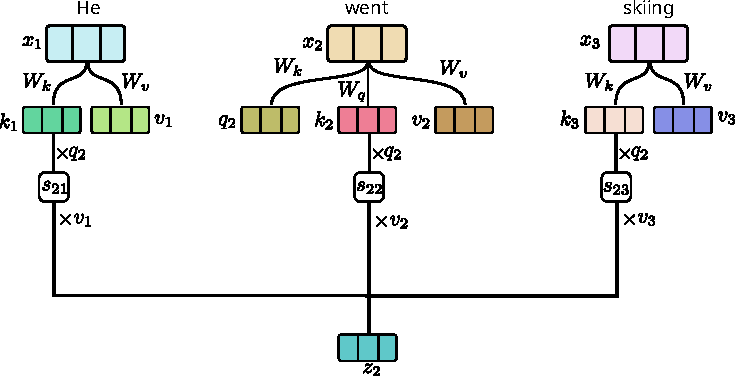
\includegraphics[scale=1.0]{./images/transformer/attention.pdf}
	\caption{An Illustration of the self-attention.}
\end{figure}

\paragraph{Input Embeddings}

   Each token \( i \) is represented by an embedding:
   \[
   \mathbf{x}_i \in \mathbb{R}^{d_{\text{model}}}.
   \]
   
   You can think of all the tokens put together as a matrix:
   \[
   X \in \mathbb{R}^{n \times d_{\text{model}}}.
   \]

\paragraph{Projection Matrices}

   To obtain the queries, keys, and values, we use learned projection matrices:
   \[
   \begin{aligned}
   W^Q &\in \mathbb{R}^{d_{\text{model}} \times d_k}, \\
   W^K &\in \mathbb{R}^{d_{\text{model}} \times d_k}, \\
   W^V &\in \mathbb{R}^{d_{\text{model}} \times d_v}.
   \end{aligned}
   \]

\paragraph{Projected Matrices}
   Multiplying the input \( X \) by these weight matrices gives:
   \[
   \begin{aligned}
   Q &= X\,W^Q \in \mathbb{R}^{n \times d_k}, \\
   K &= X\,W^K \in \mathbb{R}^{n \times d_k}, \\
   V &= X\,W^V \in \mathbb{R}^{n \times d_v}.
   \end{aligned}
   \]
   
   Here, each row of \( Q \) (or \( K \), or \( V \)) corresponds to the query (or key, or value) of one token.

\paragraph{Dot-Product Attention Scores}

   The attention scores between tokens are computed using:
   \[
   QK^\top \in \mathbb{R}^{n \times n}.
   \]
   
   In this product:
   \begin{itemize}
	   \item \( Q \) is \( n \times d_k \)
	   \item \( K^\top \) is \( d_k \times n \)
   \end{itemize}
   
   
   Therefore, the result is an \( n \times n \) matrix where each entry \((i,j)\) represents the (unnormalized) similarity between token \( i \) and token \( j \).

   \paragraph{Scaled Dot-Product and Softmax}

   Before applying the softmax, the scores are scaled by \( \sqrt{d_k} \):
   \[
   \frac{QK^\top}{\sqrt{d_k}} \in \mathbb{R}^{n \times n}.
   \]
   
   Then, applying the softmax function row-wise produces an attention weight matrix \( A \in \mathbb{R}^{n \times n} \):
   \[
   A = \operatorname{softmax}\!\left(\frac{QK^\top}{\sqrt{d_k}}\right).
   \]

   \paragraph{Final Output}
   Finally, the output of the self-attention layer is computed as:
   \[
   \text{Attention}(Q, K, V) = A\,V.
   \]
   
   Since:
   \begin{itemize}
	   \item \( A \) is \( n \times n \),
	   \item \( V \) is \( n \times d_v \),
   \end{itemize}
   
   The final output is:
   \[
   \text{Attention}(Q, K, V) \in \mathbb{R}^{n \times d_v}.
   \]

\subsection{Masked Attention}
In autoregressive tasks (\eg language modeling), it is essential that when predicting a token at position ii, the model does not ``peek'' at any tokens at positions $j>i$. \textit{Masked attention} ensures that each token only attends to tokens at the same or earlier positions. The masked attention is often referred to \textit{cross-attention}. This is just a self-attention in decoder.
$$\textrm{MA}(Q,K,V) = softmax\bigg(\frac{Q^TK+M}{\sqrt{d_k}}\bigg)V,$$
where $M$ 
\begin{align*}
	M_{ij} = \begin{cases}
		0&\text{if } j\leq i\\
		-\infty&\text{if } j>i
	\end{cases}
\end{align*}
Note that $-\infty$ will make $exp$ term to be zero.

\subsection{Multi-Head Attention}
Multi-head attention allows the model to jointly attend to information from different representation subspaces at different positions. \textbf{Rather than computing a single attention function with full-dimensional queries, keys, and values, the mechanism splits them into multiple ``heads'' and computes attention in parallel}. 

Suppose:
\begin{itemize}
	\item The input embeddings (or previous layer outputs) form the matrix \(X \in \mathbb{R}^{n \times d_{\text{model}}}\),
	\item \(d_{\text{model}}\) is the model (or embedding) dimension,
	\item We decide to use \(h\) attention heads.
\end{itemize}

Each head will work with lower-dimensional projections of the input. In particular, we typically set:
\[
d_k' = d_v' = \frac{d_{\text{model}}}{h},
\]
so that each head processes queries, keys, and values of dimensions \(d_k'\) and \(d_v'\), and the total computation remains efficient.

\paragraph{Linear Projections for Each Head}

   For each head \(i \in \{1, \dots, h\}\), we define learned projection matrices:
   \[
   \begin{aligned}
   W_i^Q &\in \mathbb{R}^{d_{\text{model}} \times d_k'}, \\
   W_i^K &\in \mathbb{R}^{d_{\text{model}} \times d_k'}, \\
   W_i^V &\in \mathbb{R}^{d_{\text{model}} \times d_v'}.
   \end{aligned}
   \]
   We then project the input \(X\) to obtain:
   \[
   \begin{aligned}
   Q_i &= X W_i^Q \in \mathbb{R}^{n \times d_k'}, \\
   K_i &= X W_i^K \in \mathbb{R}^{n \times d_k'}, \\
   V_i &= X W_i^V \in \mathbb{R}^{n \times d_v'}.
   \end{aligned}
   \]

\paragraph{Compute Scaled (Masked) Dot-Product Attention for Each Head}

   For each head \(i\), compute:
   \[
   \text{head}_i = \operatorname{Attention}(Q_i, K_i, V_i),
   \]
   where the attention function is defined as:
   \[
   \text{head}_i = \operatorname{softmax}\!\left(\frac{Q_iK_i^\top + M}{\sqrt{d_k'}}\right) V_i.
   \]
   \begin{itemize}
	   \item If masking is not required (\eg in the encoder or in \textit{non-autoregressive} settings), simply set \(M = 0\).
	   \item \textit{For decoder self-attention in autoregressive models}, \(M\) is defined as in the Masked Attention section above.
   \end{itemize}

\paragraph{Concatenate the Heads and Project}

   Once all heads are computed, we concatenate their outputs:
   \[
   \text{Concat}(\text{head}_1, \text{head}_2, \dots, \text{head}_h) \in \mathbb{R}^{n \times (h \cdot d_v')}.
   \]
   Finally, we apply a learned linear projection:
   \[
   W^O \in \mathbb{R}^{(h \cdot d_v') \times d_{\text{model}}},
   \]
   to obtain the final multi-head attention output:
   \[
   \text{MultiHead}(Q, K, V) = \text{Concat}(\text{head}_1, \dots, \text{head}_h) W^O \in \mathbb{R}^{n \times d_{\text{model}}}.
   \]

   % \begin{itemize}
		% \item Input \(X\): \( n \times d_{\text{model}} \)
		% \item Projection matrices \(W_i^Q, W_i^K, W_i^V\): \( d_{\text{model}} \times d_k' \) (or \( d_v' \))
		% \item Projected matrices for each head:
		% \item  \( Q_i, K_i \in \mathbb{R}^{n \times d_k'} \)
		% \item  \( V_i \in \mathbb{R}^{n \times d_v'} \)
		% \item Attention score matrix (per head):
		% \item \( Q_iK_i^\top \in \mathbb{R}^{n \times n} \)
		% \item Output of each head: \( \text{head}_i \in \mathbb{R}^{n \times d_v'} \)
		% \item Concatenated heads: \( n \times (h \cdot d_v') \)
		% \item Final projection \(W^O\): \( (h \cdot d_v') \times d_{\text{model}} \)
		% \item Final multi-head attention output: \( n \times d_{\text{model}} \)
   % \end{itemize}


\subsection{Variations of MHA}

\begin{figure}[t]
	\centering
	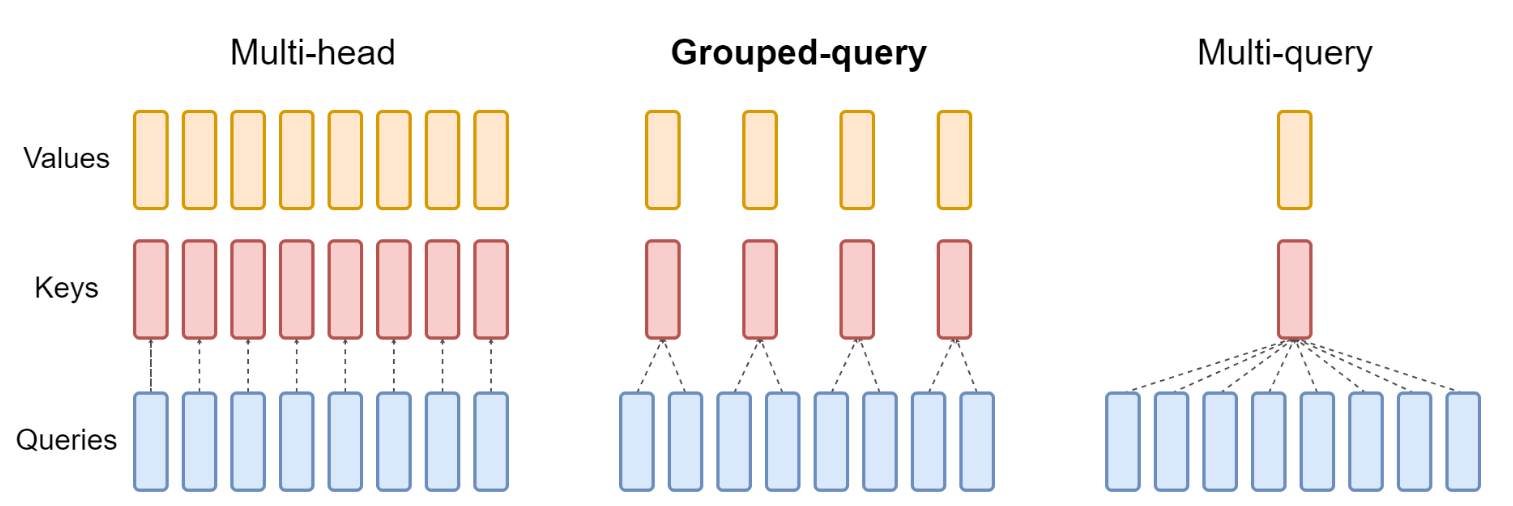
\includegraphics[scale=0.5]{./images/transformer/multi_head_attention.png}
\end{figure}

If we use a single value and a single key over all queries, we can significantly reduce the memory usage for KV caching. This is the basic idea of the multi-query attention and the grouped query attention.
   
% \subsection{Skip Connection}
% This is a regularization technique.

\section{Positional Embedding}

The self-attention mechanism in transformers treats all tokens in a sequence in parallel without an inherent notion of order. This means that, by itself, self-attention is invariant to the order of input tokens. Positional encoding is introduced to inject order information so that the model can differentiate between tokens based on their positions.

\begin{figure}[t]
	\centering
	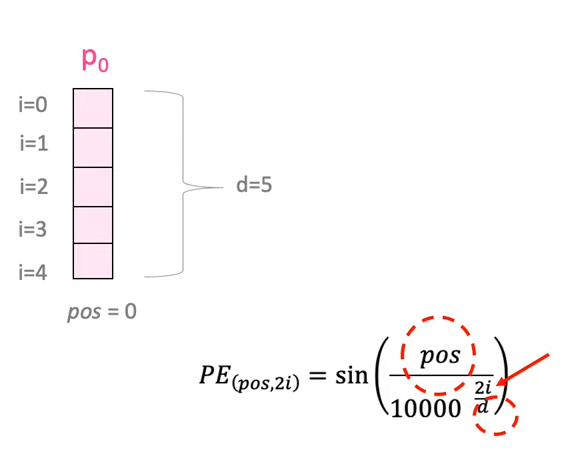
\includegraphics[scale=0.6]{./images/transformer/positional_1.png}
	\caption{Positional embedding.}
\end{figure}

\subsection{RoPE}

RoPE represents a novel approach in encoding positional information. Traditional methods, either absolute or relative, come with their limitations. Absolute positional embeddings assign a unique vector to each position, which though straightforward, doesn't scale well and fails to capture relative positions effectively. Relative embeddings, on the other hand, focus on the distance between tokens, enhancing the model’s understanding of token relationships but complicating the model architecture.

RoPE ingeniously combines the strengths of both. It encodes positional information in a way that allows the model to understand both the absolute position of tokens and their relative distances. This is achieved through a rotational mechanism, where each position in the sequence is represented by a rotation in the embedding space. The elegance of RoPE lies in its simplicity and efficiency, enabling models to better grasp the nuances of language syntax and semantics.

RoPE introduces a novel concept. Instead of adding a positional vector, it applies a rotation to the word vector. Imagine a two-dimensional word vector for ``dog.'' To encode its position in a sentence, RoPE rotates this vector. The angle of rotation ($\theta$) is proportional to the word's position in the sentence. For instance, the vector is rotated by $\theta$ for the first position, $2\theta$ for the second, and so on. This approach has several benefits

RoPE introduces position information by rotating the query and key vectors in each attention head by a position-specific angle. Each pair \((2k, 2k+1)\) of embedding dimensions corresponds to a 2D plane in which a rotation is applied. As the position index \(i\) changes, the rotation angle changes accordingly.
Let:
\begin{itemize}
	\item \( \mathbf{x}_i \in \mathbb{R}^d \) be the embedding vector (for either query \(Q\) or key \(K\)) at position \(i\).
	\item We partition \(\mathbf{x}_i\) into \(d/2\) ``complex'' components or 2D planes.  
	  Concretely, we can view \(\mathbf{x}_i\) as $(x_{i,2k}, x_{i,2k+1})$, where $k = 0, 1, \ldots, \frac{d}{2}-1$.
\end{itemize}


We define a rotation angle \(\theta_{i, k}\) for each pair of dimensions \((2k, 2k+1)\). One common choice is:
\[
\theta_{i, k} \;=\; i \cdot \alpha_k,
\]
where \(\alpha_k\) might be a scaling based on the dimension index \(k\). A popular definition (akin to sinusoidal absolute embeddings) sets:
\[
\alpha_k \;=\; \frac{1}{10000^{\frac{2k}{d}}}.
\]
For each pair \((2k, 2k+1)\), define the rotary transformation \(\text{RoPE}(\cdot)\) as follows. Let
\[
\mathbf{x}_i^{(k)} 
= \begin{pmatrix}
x_{i, 2k} \\[6pt]
x_{i, 2k+1}
\end{pmatrix}.
\]
Then,
\[
\text{RoPE}_i \bigl(\mathbf{x}_i^{(k)}\bigr)
= \begin{pmatrix}
\cos(\theta_{i, k}) & -\sin(\theta_{i, k}) \\
\sin(\theta_{i, k}) & \cos(\theta_{i, k})
\end{pmatrix}
\begin{pmatrix}
x_{i, 2k} \\[4pt]
x_{i, 2k+1}
\end{pmatrix}.
\]

Hence, the updated 2D coordinates are:

\[
\begin{aligned}
\tilde{x}_{i, 2k} &= x_{i, 2k}\,\cos(\theta_{i,k}) \;-\; x_{i, 2k+1}\,\sin(\theta_{i,k}),\\[6pt]
\tilde{x}_{i, 2k+1} &= x_{i, 2k+1}\,\cos(\theta_{i,k}) \;+\; x_{i, 2k}\,\sin(\theta_{i,k}).
\end{aligned}
\]

We perform this rotation across all \(k = 0, 1, \dots, \frac{d}{2}-1\), concatenating the results back into a \(d\)-dimensional vector \(\tilde{\mathbf{x}}_i\).

In many implementations, we apply RoPE to both the query \(\mathbf{q}_i\) and key \(\mathbf{k}_j\) vectors for each position \(i, j\). That is:
\[
\begin{aligned}
\tilde{\mathbf{q}}_i &= \text{RoPE}_i(\mathbf{q}_i), \\
\tilde{\mathbf{k}}_j &= \text{RoPE}_j(\mathbf{k}_j).
\end{aligned}
\]
Then, during the attention calculation:
\[
\text{Attention}(i, j) 
= \frac{\tilde{\mathbf{q}}_i \,\cdot\, \tilde{\mathbf{k}}_j}{\sqrt{d}}.
\]

The key property is that
\[
\tilde{\mathbf{q}}_i^\top \, \tilde{\mathbf{k}}_j
\;\;=\;\;
\mathbf{q}_i^\top\, \mathbf{M}(i,j)\, \mathbf{k}_j,
\]

where \(\mathbf{M}(i,j)\) is a matrix encoding the position difference \((i-j)\). This yields a relative-positional effect without explicitly storing or adding embedding vectors for each position pair.


\begin{itemize}
	\item Stability of Vectors: Adding tokens at the end of a sentence doesn't affect the vectors for words at the beginning, facilitating efficient caching.
		\item Preservation of Relative Positions: If two words, say ``pig'' and ``dog,'' maintain the same relative distance in different contexts, their vectors are rotated by the same amount. This ensures that the angle, and consequently the dot product between these vectors, remains constant
\end{itemize}

## Rotary Positional Encoding (RoPE): A Comprehensive Explanation

### **Background: Why Positional Encoding Matters**

In transformer models, the self-attention mechanism treats all tokens as a set without any inherent order. However, many tasks (like language processing) depend on the sequential order of tokens. Traditional methods to incorporate this order include:

- **Absolute Positional Embeddings:**  
  Each position in the sequence is assigned a unique vector. Although straightforward, these embeddings don’t scale well to longer sequences and fail to capture the nuances of relative positions between tokens.

- **Relative Positional Embeddings:**  
  These embeddings focus on the distance between tokens, which can improve the model’s understanding of token relationships. However, they typically introduce additional complexity into the model architecture.

**RoPE cleverly combines the strengths of both approaches** by encoding position information directly into the query and key vectors using a rotation-based mechanism. This approach allows the model to capture both the absolute positions of tokens and the relative differences between them without adding extra learned parameters for position.

---

### **The Core Idea of RoPE**

Rather than adding a positional vector to the token embeddings, RoPE **rotates** the embeddings by a position-specific angle. Think of it as "twisting" the embedding in space based on its position. For example, if you have a simple two-dimensional embedding for the word “dog,” you can imagine its vector being rotated by an angle \(\theta\) if it’s the first word, \(2\theta\) if it’s the second word, and so on.

#### **Decomposing High-Dimensional Embeddings into 2D Subspaces**

For high-dimensional embeddings (say, in \(\mathbb{R}^d\)), RoPE divides the vector into \(d/2\) pairs (or 2D subspaces). For a token at position \(i\), denote its embedding by:
\[
\mathbf{x}_i \in \mathbb{R}^d.
\]
We partition \(\mathbf{x}_i\) into pairs:
\[
\mathbf{x}_i^{(k)} = 
\begin{pmatrix}
x_{i,2k} \\
x_{i,2k+1}
\end{pmatrix},\quad k = 0, 1, \ldots, \frac{d}{2}-1.
\]

#### **Defining the Rotation Angle**

For each 2D subspace indexed by \(k\), RoPE defines a rotation angle:
\[
\theta_{i, k} = i \cdot \alpha_k,
\]
where \(\alpha_k\) is a scaling factor that typically depends on the dimension \(k\). A popular choice is:
\[
\alpha_k = \frac{1}{10000^{\frac{2k}{d}}}.
\]
This scaling mimics the frequency scaling in sinusoidal embeddings, ensuring that different subspaces capture positional information at different granularities.

---

### **Where Does \(R(\theta)\) Come From?**

In two-dimensional geometry, any rotation by an angle \(\theta\) can be represented by a **rotation matrix** \(R(\theta)\). This matrix is a standard tool in linear algebra and has the form:
\[
R(\theta) = 
\begin{pmatrix}
\cos(\theta) & -\sin(\theta) \\
\sin(\theta) & \cos(\theta)
\end{pmatrix}.
\]

**Why use \(R(\theta)\)?**  
- **Geometric Interpretation:**  
  The rotation matrix \(R(\theta)\) rotates any 2D vector by the angle \(\theta\) (in the counterclockwise direction) while preserving its magnitude. This property makes it ideal for encoding positional shifts—rotating a vector does not change its “content” (its norm) but changes its direction, thereby encoding positional information.
  
- **Simplicity and Efficiency:**  
  Because the rotation matrix is defined entirely by trigonometric functions (which are computationally efficient), it adds minimal overhead to the model.

- **Inherent Relative Encoding:**  
  When different positions correspond to different rotation angles, the relationship between any two positions can be captured by the difference in their rotation angles. This leads to a natural encoding of relative position without having to explicitly compute or store separate relative position vectors.

---

### **Applying RoPE to Token Embeddings**

For each 2D subspace, the rotary transformation is applied as follows. Given the subvector:
\[
\mathbf{x}_i^{(k)} = 
\begin{pmatrix}
x_{i,2k} \\
x_{i,2k+1}
\end{pmatrix},
\]
we compute its rotated version:
\[
\text{RoPE}_i \bigl(\mathbf{x}_i^{(k)}\bigr)
= R(\theta_{i, k})\, \mathbf{x}_i^{(k)}
= \begin{pmatrix}
\cos(\theta_{i, k}) & -\sin(\theta_{i, k}) \\
\sin(\theta_{i, k}) & \cos(\theta_{i, k})
\end{pmatrix}
\begin{pmatrix}
x_{i,2k} \\
x_{i,2k+1}
\end{pmatrix}.
\]
This yields the updated coordinates:
\[
\begin{aligned}
\tilde{x}_{i, 2k} &= x_{i,2k}\cos(\theta_{i,k}) - x_{i,2k+1}\sin(\theta_{i,k}),\\[6pt]
\tilde{x}_{i, 2k+1} &= x_{i,2k+1}\cos(\theta_{i,k}) + x_{i,2k}\sin(\theta_{i,k}).
\end{aligned}
\]
After processing all \(d/2\) subspaces, we concatenate the results back into a full \(d\)-dimensional vector \(\tilde{\mathbf{x}}_i\).

---

### **Integration into the Self-Attention Mechanism**

In transformer architectures, RoPE is applied to both the query and key vectors:

\[
\begin{aligned}
\tilde{\mathbf{q}}_i &= \text{RoPE}_i(\mathbf{q}_i), \\
\tilde{\mathbf{k}}_j &= \text{RoPE}_j(\mathbf{k}_j).
\end{aligned}
\]

Then, the attention score between positions \(i\) and \(j\) is calculated as:
\[
\text{Attention}(i, j) = \frac{\tilde{\mathbf{q}}_i \cdot \tilde{\mathbf{k}}_j}{\sqrt{d}}.
\]

---

### **Understanding the Matrix \(\mathbf{M}(i,j)\) and Its Connection to \(R(\theta)\)**

A key property of RoPE is that the dot product between the rotated vectors can be reinterpreted to show how relative positions are encoded. In particular, one can derive that:
\[
\tilde{\mathbf{q}}_i^\top \tilde{\mathbf{k}}_j = \mathbf{q}_i^\top\, \mathbf{M}(i,j)\, \mathbf{k}_j,
\]
where \(\mathbf{M}(i,j)\) is a block diagonal matrix that encapsulates the effect of the relative positional difference \(j-i\).

#### **Derivation in a Single 2D Subspace**

Focus on one 2D subspace (indexed by \(k\)):
- The query subvector at position \(i\) is rotated by \(\theta_{i,k} = i\alpha_k\).
- The key subvector at position \(j\) is rotated by \(\theta_{j,k} = j\alpha_k\).

The dot product in this subspace is:
\[
\tilde{\mathbf{q}}_i^{(k)\top} \tilde{\mathbf{k}}_j^{(k)} 
= \left(\mathbf{q}_i^{(k)}\right)^\top R(\theta_{i,k})^\top R(\theta_{j,k}) \, \mathbf{k}_j^{(k)}.
\]
Since the transpose of a rotation matrix is its inverse (i.e., \(R(\theta)^\top = R(-\theta)\)), we have:
\[
R(\theta_{i,k})^\top R(\theta_{j,k}) = R(-\theta_{i,k})R(\theta_{j,k}) = R\bigl(\theta_{j,k} - \theta_{i,k}\bigr).
\]
Because \(\theta_{j,k} - \theta_{i,k} = (j-i)\alpha_k\), the transformation becomes:
\[
R\bigl((j-i)\alpha_k\bigr).
\]

#### **Constructing \(\mathbf{M}(i,j)\)**

Repeating this for each 2D subspace results in a block diagonal matrix:
\[
\mathbf{M}(i,j) = \text{diag}\Bigl(
R\bigl((j-i)\alpha_0\bigr),\,
R\bigl((j-i)\alpha_1\bigr),\,
\ldots,\,
R\bigl((j-i)\alpha_{\frac{d}{2}-1}\bigr)
\Bigr).
\]
Each block is the 2×2 rotation matrix:
\[
R\bigl((j-i)\alpha_k\bigr)
= \begin{pmatrix}
\cos\bigl((j-i)\alpha_k\bigr) & -\sin\bigl((j-i)\alpha_k\bigr) \\
\sin\bigl((j-i)\alpha_k\bigr) & \cos\bigl((j-i)\alpha_k\bigr)
\end{pmatrix}.
\]

#### **Intuition Behind \(\mathbf{M}(i,j)\)**

- **Relative Positional Bias:**  
  The matrix \(\mathbf{M}(i,j)\) adjusts the dot product between queries and keys based on their relative positions \((j-i)\). Instead of explicitly adding a relative position embedding, the rotation inherently modulates the interaction between tokens.
  
- **Unified Encoding:**  
  Because \(\mathbf{M}(i,j)\) is built from standard rotation matrices \(R(\theta)\), it seamlessly encodes the relative positional difference across all 2D subspaces. This results in a unified treatment where both absolute and relative positional cues are embedded into the attention calculation.
  
- **Elegant Mathematical Foundation:**  
  The use of \(R(\theta)\) comes directly from classical geometry and linear algebra. It leverages the well-known properties of rotations in 2D—specifically, that rotations preserve vector norms and that the composition of rotations is itself a rotation (with the angle being the sum or difference of the individual angles). This mathematical elegance translates into an efficient and effective mechanism for positional encoding.

---

### **Summary**

1. **Rotary Positional Encoding (RoPE)** rotates the token embeddings by a position-dependent angle rather than simply adding a positional vector.
2. **Decomposition into 2D Subspaces:**  
   The \(d\)-dimensional embedding is split into \(d/2\) pairs. For each pair (treated as a 2D vector), a rotation is applied.
3. **Rotation Matrix \(R(\theta)\):**  
   The standard 2D rotation matrix,
   \[
   R(\theta) = 
   \begin{pmatrix}
   \cos(\theta) & -\sin(\theta) \\
   \sin(\theta) & \cos(\theta)
   \end{pmatrix},
   \]
   rotates vectors by \(\theta\) and comes from classical geometry. It is used here because it naturally encodes a continuous positional shift.
4. **Position-Specific Rotation:**  
   For token at position \(i\) in subspace \(k\), the rotation angle is \(\theta_{i, k} = i \cdot \alpha_k\), where \(\alpha_k\) scales the rotation differently for each subspace.
5. **Integration with Attention:**  
   RoPE is applied to both query and key vectors. The dot product between rotated vectors can be re-expressed as:
   \[
   \tilde{\mathbf{q}}_i^\top \tilde{\mathbf{k}}_j = \mathbf{q}_i^\top\, \mathbf{M}(i,j)\, \mathbf{k}_j,
   \]
   where \(\mathbf{M}(i,j)\) is a block diagonal matrix with blocks \(R((j-i)\alpha_k)\) that capture the relative position between tokens.

By rotating the embeddings with \(R(\theta)\), RoPE introduces a sophisticated yet efficient mechanism to encode both absolute and relative positional information, enhancing the transformer’s ability to capture the structure and nuances inherent in sequential data.


\begin{lstlisting}[language=Python]
def position_encoding(seq_len: int, dim_model: int)->Tensor:
    pos = torch.arange(seq_len, dtype=torch.float).reshape(1, -1, 1)
    dim = torch.arange(dim_model, dtype=torch.float).reshape(1, 1, -1)
    phase = pos / (1e4 ** (dim // dim_model))
    return torch.where(dim.long() % 2 == 0, torch.sin(phase), torch.cos(phase))
\end{lstlisting}


\subsection{Encoder}

\subsection{Decoder}
The output of each step is fed to the bottom decoder in the next time step, and the decoders bubble up their decoding results just like the encoders did. And just like we did with the encoder inputs, we embed and add positional encoding to those decoder inputs to indicate the position of each word.

\begin{lstlisting}[language=Python]
def forward(self, tgt: Tensor, memory: Tensor) -> Tensor:
	seq_len, dimension = tgt.size(1), tgt.size(2)
	tgt += position_encoding(seq_len, dimension)
	for layer in self.layers:
		tgt = layer(tgt, memory)
	return torch.softmax(self.linear(tgt), dim=-1)
\end{lstlisting}


\section{Inference of Autoregressive Model}

In an autoregressive transformer (such as GPT), tokens are generated one at a time. During inference, the model must compute attention for the next token based on all previously generated tokens. However, because recomputing the entire attention from scratch at each time step would be inefficient, these models use \textit{caching} to store intermediate results (the keys and values) from previous time steps. Below is an explanation with equations and clear notations.

\paragraph{Inference Overview in Autoregressive Models}
\begin{itemize}
	\item Training: The model can process the entire sequence in parallel using masked self-attention. A mask (typically a triangular matrix) prevents tokens from ``seeing'' future tokens.
	\item Inference: The model generates one token at a time. At time step \( t+1 \), it uses the already generated tokens \( [x_1, x_2, \dots, x_t] \) to compute the probability distribution for the next token.
\end{itemize}

To avoid recomputing keys and values for tokens \( x_1, \dots, x_t \) at every step, the model stores them (usually for each layer). When a new token is generated, only its query needs to be computed, and then the cached keys and values are used to compute the attention.

The technique of storing and reusing the computed keys and values from previous tokens during autoregressive generation is commonly called \textit{KV caching} (short for Key-Value Caching).

\paragraph{Step 1: Previous Tokens and Cached Representations}

Assume that by time step \( t \) the model has generated tokens:
\[
x_1,\, x_2,\, \dots,\, x_t.
\]

For a given transformer layer, let the cached key and value matrices be:
\[
\begin{aligned}
K_{\leq t} &\in \mathbb{R}^{t \times d_k}, \\
V_{\leq t} &\in \mathbb{R}^{t \times d_v},
\end{aligned}
\]
where \( d_k \) is the key (and query) dimension and \( d_v \) is the value dimension.

\paragraph{Step 2: Compute the Query for the New Token}

When generating the next token \( x_{t+1} \), its input (often the embedding of the previously generated token or a special “start” symbol) is used to compute a query vector for each layer:
\[
q_{t+1} \in \mathbb{R}^{d_k}.
\]

This is computed by a linear projection:
\[
q_{t+1} = x_{t+1} \, W^Q,
\]
where \( W^Q \in \mathbb{R}^{d_{\text{model}} \times d_k} \) is the learned projection matrix.

\paragraph{Step 3: Compute the Attention Scores}

The new query \( q_{t+1} \) is compared with all the cached keys. In a single attention head, the (scaled) dot-product attention scores are computed as:
\[
s_{t+1,j} = \frac{q_{t+1} \cdot k_j}{\sqrt{d_k}} \quad \text{for } j=1,2,\dots,t,
\]
and often, for implementation convenience, the new token's own key \( k_{t+1} \) is also computed and appended to the cache. In that case, you would have:
\[
s_{t+1,j} = \frac{q_{t+1} \cdot k_j}{\sqrt{d_k}} \quad \text{for } j=1,2,\dots,t+1.
\]

Since the model is autoregressive, the mask is implicit. There are no ``future'' tokens beyond \( t+1 \) at inference time. (If you do compute for all \( t+1 \) positions, a mask would ensure that token \( t+1 \) only attends to tokens \( 1 \) through \( t+1 \).)

\paragraph{Step 4: Apply the Softmax to Get Attention Weights}

The scores are then normalized with the softmax function to obtain the attention weights:
\[
\alpha_{t+1,j} = \frac{\exp(s_{t+1,j})}{\sum_{j'=1}^{t+1} \exp(s_{t+1,j'})}, \quad j = 1,\dots,t+1.
\]

These weights determine how much the new token attends to each of the previous tokens (and its own representation, if included).

\paragraph{Step 5: Compute the Weighted Sum of Values}

The output of the attention layer for the new token is then computed as:
\[
z_{t+1} = \sum_{j=1}^{t+1} \alpha_{t+1,j}\, v_j,
\]
where each \( v_j \) is the value vector from the cache (or computed for the new token in the case of \( j=t+1 \)):
\[
v_j = x_j\, W^V, \quad j = 1,\dots,t+1.
\]

This \( z_{t+1} \) is then passed on through the rest of the transformer layer (including feed-forward sub-layers, layer normalization, etc.) to eventually produce logits over the vocabulary.

\paragraph{Step 6: Generate the Next Token and Update the Cache}
\begin{itemize}
	\item The model uses the final output (after all transformer layers) to compute a probability distribution over the vocabulary.
	\item A token is chosen (\eg via sampling or greedy decoding) and appended to the sequence.
	\item The new token's key and value vectors (from each layer) are computed and added to the cache so that future tokens can attend to it.
\end{itemize}

\subsection{Inference without Caching}

Let's take a look at the following example:
\begin{itemize}
	\item Number of tokens so far: \(t=3\). We have already generated tokens \(\{x_1, x_2, x_3\}\). We now want to generate token \(x_4\).  
	\item Model dimensionality: To keep it simple, let's say each token embedding is 2-dimensional (\(d_{\text{model}} = 2\)) and the attention uses a single head with key/query dimension \(d_k = 2\) and value dimension \(d_v = 2\). 
	\item Token embeddings (just made-up numbers):
	  \[
		x_1 = \begin{bmatrix}1 \\ 2\end{bmatrix}, \quad
		x_2 = \begin{bmatrix}3 \\ 4\end{bmatrix}, \quad
		x_3 = \begin{bmatrix}5 \\ 6\end{bmatrix}, \quad
		x_4 = \begin{bmatrix}? \\ ?\end{bmatrix} \; 
	  \]
	  The forth one is the one we want to generate. We will compute attention for tokens \(x_1, x_2, x_3, x_4\) all at once.  
  \item Projection matrices (\(W^Q, W^K, W^V\)) are each \(2 \times 2\) for this example. For instance, we have the following matrices:
  \[
    W^Q = \begin{bmatrix}1 & 0 \\[6pt] 0 & 1\end{bmatrix}, \quad
    W^K = \begin{bmatrix}1 & 2 \\[6pt] 0 & 1\end{bmatrix}, \quad
    W^V = \begin{bmatrix}0.5 & -0.5 \\[6pt] 1.0 & 0.5\end{bmatrix}.
  \]
\end{itemize}

\paragraph{Step A: Compute Queries, Keys, and Values}

\begin{itemize}
	\item Queries:  
   \[
     q_i = x_i \, W^Q 
   \]
   For \(i=1,2,3,4\):
   \begin{itemize}
	   \item \(q_1 = [1\;\;2] \begin{bmatrix}1 & 0 \\ 0 & 1\end{bmatrix} = \begin{bmatrix}1 \\ 2\end{bmatrix}\)
	   \item \(q_2 = [3\;\;4] \begin{bmatrix}1 & 0 \\ 0 & 1\end{bmatrix} = \begin{bmatrix}3 \\ 4\end{bmatrix}\)
	   \item \(q_3 = [5\;\;6] \begin{bmatrix}1 & 0 \\ 0 & 1\end{bmatrix} = \begin{bmatrix}5 \\ 6\end{bmatrix}\)
	   \item \(q_4 = [?,\; ?] \begin{bmatrix}1 & 0 \\ 0 & 1\end{bmatrix} = \begin{bmatrix}? \\ ?\end{bmatrix}\)
   \end{itemize}
	\item Keys:
	   \[
		 k_i = x_i \, W^K
	   \]
	   For \(i=1,2,3,4\):
	   \begin{itemize}
		   \item \(k_1 = [1\;\;2] \begin{bmatrix}1 & 2 \\ 0 & 1\end{bmatrix}
			 = \begin{bmatrix}1 \\ 4\end{bmatrix}\)
		   \item \(k_2 = [3\;\;4] \begin{bmatrix}1 & 2 \\ 0 & 1\end{bmatrix} 
			 = \begin{bmatrix}3 \\ 10\end{bmatrix}\)
		   \item \(k_3 = [5\;\;6] \begin{bmatrix}1 & 2 \\ 0 & 1\end{bmatrix} 
			 = \begin{bmatrix}5 \\ 16\end{bmatrix}\)
		   \item \(k_4 = [?,\; ?] \begin{bmatrix}1 & 2 \\ 0 & 1\end{bmatrix} 
			 = \begin{bmatrix}? \\ ?\end{bmatrix}\)
	   \end{itemize}
	\item Values:
	   \[
		 v_i = x_i \, W^V
	   \]
	   For \(i=1,2,3,4\):
	   \begin{itemize}
		   \item \(v_1 = [1\;\;2] \begin{bmatrix}0.5 & -0.5 \\ 1.0 & 0.5\end{bmatrix} 
			 = \begin{bmatrix}2.5 \\ 0.5\end{bmatrix}\)
		   \item \(v_2 = [3\;\;4] \begin{bmatrix}0.5 & -0.5 \\ 1.0 & 0.5\end{bmatrix} 
			 = \begin{bmatrix}5.5 \\ 0.5\end{bmatrix}\)
		   \item \(v_3 = [5\;\;6] \begin{bmatrix}0.5 & -0.5 \\ 1.0 & 0.5\end{bmatrix} 
			 = \begin{bmatrix}8.5 \\ 0.5\end{bmatrix}\)
		   \item \(v_4 = [?,\; ?] \begin{bmatrix}0.5 & -0.5 \\ 1.0 & 0.5\end{bmatrix} 
			 = \begin{bmatrix}? \\ ?\end{bmatrix}\)
	   \end{itemize}
\end{itemize}

All of the above must be computed at the current time step if we do not use caching.

With KV caching, you would \emph{not} recalculate \(k_1, k_2, k_3\) and \(v_1, v_2, v_3\). Instead:

\begin{itemize}
	\item You already have \(\{k_1, k_2, k_3\}\) and \(\{v_1, v_2, v_3\}\) stored from the previous steps.  
	\item You only compute:
		\begin{itemize}
			\item \(q_4\) (the query for the new token),
			\item \(k_4, v_4\) (the new key and value to add to the cache).  
		\end{itemize}
\end{itemize}
In other words, you skip re-projecting and re-computing every key and value from tokens \(\{1,2,3\}\). This saves a substantial amount of computation when generating long sequences, especially in large transformers (like GPT).

\textbf{Note that storing data in the cache uses up memory space.} Systems with limited memory resources may struggle to accommodate this additional memory overhead, potentially resulting in out-of-memory errors. This is especially the case when long inputs need to be processed, as the memory required for the cache grows linearly with the input length and the batch size.

\paragraph{Summary}
\begin{itemize}
	\item Without caching, each step of generation must feed the entire partial sequence \(\{x_1, \ldots, x_t\}\) through all attention layers, resulting in \(\mathcal{O}(t)\) computations per token. Doing that for each of the \(t\) tokens leads to \(\mathcal{O}(t^2)\) complexity for generating \(t\) tokens.
	\item With caching, the complexity for each new token is \(\mathcal{O}(1)\) on the transformer's forward pass for the new key/value (plus the cost of computing attention of dimension \(\mathcal{O}(t)\) for the new query). Overall, this significantly speeds up autoregressive decoding.
\end{itemize}


\begin{figure}[t]
	\centering
	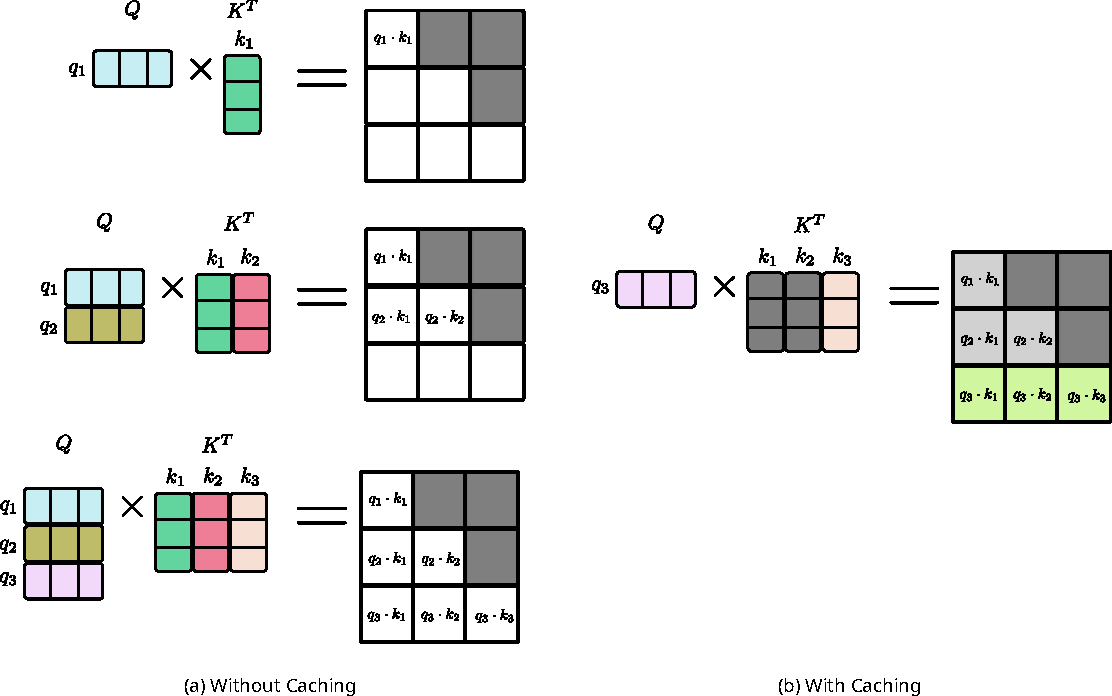
\includegraphics[scale=0.8]{./images/transformer/kv_caching.pdf}
\end{figure}

